\documentclass[12pt]{article}
\usepackage{amsmath}
\usepackage{amssymb}
\usepackage{geometry}
\usepackage{enumitem}
\usepackage{listings}
\usepackage{xcolor}
\usepackage{tikz}
\usetikzlibrary{shapes.geometric, arrows}
\geometry{a4paper, margin=1in}

% Python code styling
\definecolor{codegreen}{rgb}{0,0.6,0}
\definecolor{codegray}{rgb}{0.5,0.5,0.5}
\definecolor{codepurple}{rgb}{0.58,0,0.82}
\definecolor{backcolour}{rgb}{0.95,0.95,0.92}

\lstdefinestyle{mystyle}{
    backgroundcolor=\color{backcolour},   
    commentstyle=\color{codegreen},
    keywordstyle=\color{magenta},
    numberstyle=\tiny\color{codegray},
    stringstyle=\color{codepurple},
    basicstyle=\ttfamily\footnotesize,
    breakatwhitespace=false,         
    breaklines=true,                 
    captionpos=b,                    
    keepspaces=true,                 
    numbers=left,                    
    numbersep=5pt,                  
    showspaces=false,                
    showstringspaces=false,
    showtabs=false,                  
    tabsize=2
}

\lstset{style=mystyle}

\begin{document}

\begin{center}
    \textbf{University of Eswatini} \\
    \textbf{Department of Computer Science} \\
    \textbf{Examination Solutions Manual} \\
    2025/2026 \\
    \textbf{FIRST SEMESTER} \\
    \vspace{1cm}
    \textbf{Title: INTRODUCTION TO COMPUTER SCIENCE} \\
    \textbf{Course Code: CSC111} \\
\end{center}

\section*{SECTION A: COMPULSORY - SOLUTIONS}

\begin{enumerate}[left=0pt, label=\bfseries Q\arabic*., start=1]
    \item \textbf{Computer Science Fundamentals} \hfill (10 marks)\\
    \textbf{Solution:} The five distinct computing disciplines identified by ACM are:
    \begin{enumerate}[label=(\alph*)]
        \item \textbf{Computer Engineering (CE)}: Design and construction of computers and computer-based systems with focus on hardware, software, and communications.
        \item \textbf{Computer Science (CS)}: Wide-ranging field from theoretical foundations to cutting-edge developments, providing comprehensive foundation for adaptability.
        \item \textbf{Information Systems (IS)}: Integration of IT solutions with business processes to meet organizational needs effectively.
        \item \textbf{Information Technology (IT)}: Meeting user needs through selection, creation, and administration of computing technologies.
        \item \textbf{Software Engineering (SE)}: Developing reliable, efficient, and affordable software systems using engineering principles.
    \end{enumerate}

    \item \textbf{Computer Generations} \hfill (10 marks)\\
    \textbf{Solution:}
    \begin{enumerate}[label=(\alph*)]
        \item \textbf{First Generation (1940-1956)}: Used vacuum tubes, magnetic drums for memory, were room-sized, programmed in machine language, generated tremendous heat, and were very expensive.
        \item \textbf{Second Generation (1956-1963)}: Used transistors instead of vacuum tubes, introduced assembly languages and high-level languages (COBOL, FORTRAN), still large but more reliable.
        \item \textbf{Third Generation (1964-1971)}: Used integrated circuits (ICs), introduced keyboards and monitors, operating systems appeared, enabled multitasking.
        \item \textbf{Fourth Generation (1971-Present)}: Uses microprocessors (thousands of circuits on a chip), led to personal computers, networks, and the internet.
        \item \textbf{Fifth Generation (Present-Beyond)}: Based on artificial intelligence, uses parallel processing, superconductors, and quantum computation, still in development.
    \end{enumerate}

    \item \textbf{System Development Life Cycle (SDLC)} \hfill (10 marks)\\
    \textbf{Solution:} The six phases of SDLC are:
    \begin{enumerate}[label=(\alph*)]
        \item \textbf{Preliminary Investigation}: Conduct preliminary analysis, propose alternatives, describe costs/benefits, submit plan (feasibility study).
        \item \textbf{Systems Analysis}: Gather data, analyze data, write report describing what system does and should do.
        \item \textbf{Systems Design}: Do preliminary design, then detailed design, write report with specifications.
        \item \textbf{Systems Development}: Acquire software and hardware, test the complete system.
        \item \textbf{System Implementation}: Coordinate to make system workable and successful, ensure user acceptance.
        \item \textbf{System Maintenance}: Conduct audits, periodic evaluations, make changes based on new conditions.
    \end{enumerate}

    \item \textbf{Computer Literacy and Professionals} \hfill (10 marks)\\
    \textbf{Solution:}
    \begin{enumerate}[label=(\alph*)]
        \item \textbf{Difference between Computer Literacy and Computer Competency}:
        \begin{itemize}
            \item \textbf{Computer Literacy}: Understanding what a computer is and how it can be used as a resource.
            \item \textbf{Computer Competency}: Applying computer skills to meet information needs and improve productivity.
        \end{itemize}
        \item \textbf{Difference between Computer Professional and Computer User}:
        \begin{itemize}
            \item \textbf{Computer Professional}: Has deep technical knowledge, focuses on system design/development, creates technical solutions. \textit{Examples}: Software Engineer, Database Administrator.
            \item \textbf{Computer User}: Has basic operational knowledge, focuses on application usage, uses existing solutions. \textit{Examples}: Accountant, Administrative Clerk.
        \end{itemize}
    \end{enumerate}

    \item \textbf{Binary Arithmetic and Storage} \hfill (10 marks)\\
    \textbf{Solution:}
    \begin{enumerate}[label=(\alph*)]
        \item $101101_2 = 1\times2^5 + 0\times2^4 + 1\times2^3 + 1\times2^2 + 0\times2^1 + 1\times2^0 = 32 + 0 + 8 + 4 + 0 + 1 = 45_{10}$
        \item $A3F_{16} = A\times16^2 + 3\times16^1 + F\times16^0 = 10\times256 + 3\times16 + 15\times1 = 2560 + 48 + 15 = 2623_{10}$\\
        In binary: $A_{16}=1010_2$, $3_{16}=0011_2$, $F_{16}=1111_2$, so $A3F_{16} = 101000111111_2$
        \item $2.5\ \text{GB} = 2.5 \times 1024\ \text{MB} = 2560\ \text{MB}$
    \end{enumerate}
\end{enumerate}

\newpage

\section*{SECTION B - SOLUTIONS}

\begin{enumerate}[left=0pt, label=\bfseries Q\arabic*., start=1]
    \item \textbf{Algorithms and Flowcharts} \hfill (15 marks)\\
    \textbf{Solution:}
    \begin{enumerate}[label=(\alph*)]
        \item \textbf{Definition}: An algorithm is a step-by-step or sequential order of solving a problem or accomplishing a task.\\
        \textbf{Characteristics}:
        \begin{enumerate}[label=\roman*.]
            \item Must have a beginning and an end
            \item Must be simple/clear for easy understanding
            \item Must have an input
            \item Must have an end result (desired output)
            \item Must be efficient and effective
        \end{enumerate}
        
        \item \textbf{Algorithm to calculate area and circumference of a circle}:
        \begin{verbatim}
Step 1: Start
Step 2: Input radius R
Step 3: Calculate area = π * R * R
Step 4: Calculate circumference = 2 * π * R
Step 5: Print area, circumference
Step 6: Stop
        \end{verbatim}
        
        \item \textbf{Flowchart for finding largest of three numbers}:
        \begin{center}
        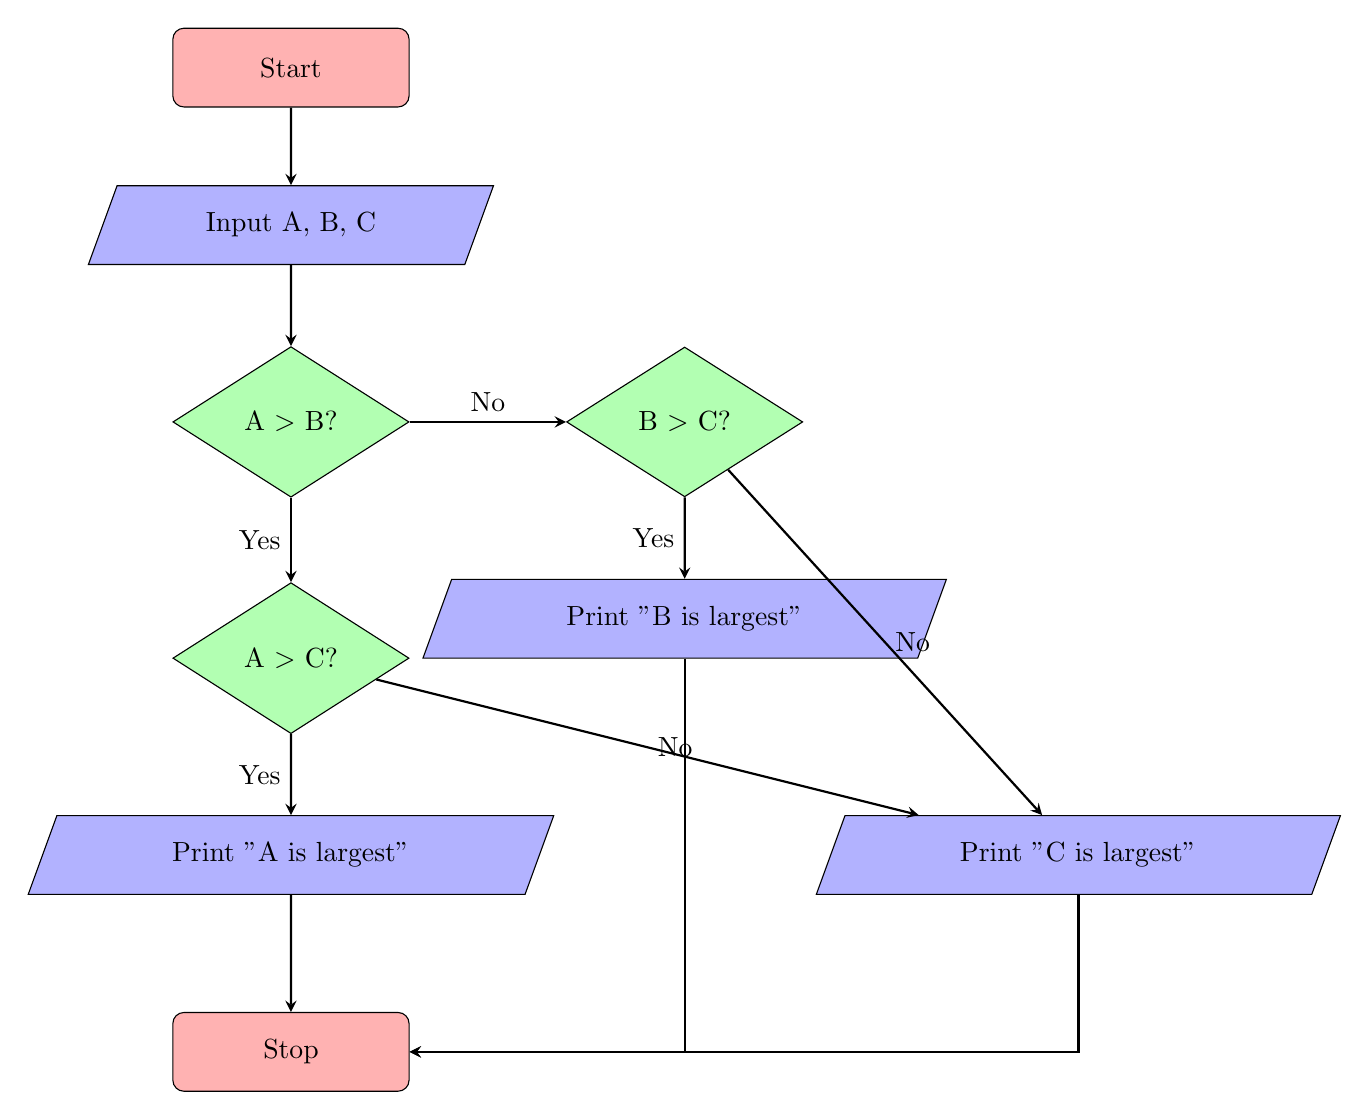
\begin{tikzpicture}[node distance=2cm]
        \tikzstyle{startstop} = [rectangle, rounded corners, minimum width=3cm, minimum height=1cm,text centered, draw=black, fill=red!30]
        \tikzstyle{io} = [trapezium, trapezium left angle=70, trapezium right angle=110, minimum width=3cm, minimum height=1cm, text centered, draw=black, fill=blue!30]
        \tikzstyle{process} = [rectangle, minimum width=3cm, minimum height=1cm, text centered, draw=black, fill=orange!30]
        \tikzstyle{decision} = [diamond, minimum width=3cm, minimum height=1cm, text centered, draw=black, fill=green!30]
        \tikzstyle{arrow} = [thick,->,>=stealth]
        
        \node (start) [startstop] {Start};
        \node (in1) [io, below of=start] {Input A, B, C};
        \node (dec1) [decision, below of=in1, yshift=-0.5cm] {A $>$ B?};
        \node (dec2) [decision, below of=dec1, yshift=-1cm] {A $>$ C?};
        \node (dec3) [decision, right of=dec1, xshift=3cm] {B $>$ C?};
        \node (out1) [io, below of=dec2, yshift=-0.5cm] {Print "A is largest"};
        \node (out2) [io, below of=dec3, yshift=-0.5cm] {Print "B is largest"};
        \node (out3) [io, right of=dec3, xshift=3cm, yshift=-5.5cm] {Print "C is largest"};
        \node (stop) [startstop, below of=out1, yshift=-0.5cm] {Stop};
        
        \draw [arrow] (start) -- (in1);
        \draw [arrow] (in1) -- (dec1);
        \draw [arrow] (dec1) -- node[anchor=east] {Yes} (dec2);
        \draw [arrow] (dec1) -- node[anchor=south] {No} (dec3);
        \draw [arrow] (dec2) -- node[anchor=east] {Yes} (out1);
        \draw [arrow] (dec2) -- node[anchor=west] {No} (out3);
        \draw [arrow] (dec3) -- node[anchor=east] {Yes} (out2);
        \draw [arrow] (dec3) -- node[anchor=west] {No} (out3);
        \draw [arrow] (out1) -- (stop);
        \draw [arrow] (out2) |- (stop);
        \draw [arrow] (out3) |- (stop);
        \end{tikzpicture}
        \end{center}
    \end{enumerate}

    \item \textbf{Python Programming I} \hfill (15 marks)\\
    \textbf{Solution:}
    \begin{enumerate}[label=(\alph*)]
        \item \textbf{Area of triangle program}:
        \begin{lstlisting}[language=Python]
# Program to calculate area of triangle
base = float(input("Enter base of triangle: "))
height = float(input("Enter height of triangle: "))
area = 0.5 * base * height
print(f"Area of triangle = {area}")
        \end{lstlisting}
        
        \item \textbf{String manipulation program}:
        \begin{lstlisting}[language=Python]
# String manipulation program
text = input("Enter a string: ")
print(f"Uppercase: {text.upper()}")
print(f"Lowercase: {text.lower()}")
print(f"Length: {len(text)}")
if len(text) >= 2:
    print(f"Without first and last characters: {text[1:-1]}")
else:
    print("String too short to remove first and last characters")
        \end{lstlisting}
    \end{enumerate}

    \item \textbf{Systems Analysis and Design} \hfill (20 marks)\\
    \textbf{Solution:}
    \begin{enumerate}[label=(\alph*)]
        \item \textbf{System definition}: A collection of related subsystems or components that interact to perform a task in order to accomplish a goal.\\
        \textbf{Key elements}:
        \begin{enumerate}[label=\roman*.]
            \item Inputs and Outputs
            \item Processor(s)
            \item Control
            \item Feedback
            \item Environment
            \item Boundaries and Interface
        \end{enumerate}
        
        \item \textbf{Reasons systems fail}:
        \begin{enumerate}[label=\roman*.]
            \item Lack of communication among users, management, and information specialists
            \item Politics and interpersonal manipulation in project environment
            \item Lack of management support
            \item Technological incompetence of people working on project
            \item Lack of user training
        \end{enumerate}
        
        \item \textbf{Importance of documentation}:
        \begin{enumerate}[label=\roman*.]
            \item To aid analysis and system understanding
            \item To aid design and development process
            \item To aid communication among team members
            \item To aid control and system management
            \item To aid training and learning for new users
            \item For future developments and enhancements
            \item For maintenance and troubleshooting
            \item For users consumption as manuals and guides
        \end{enumerate}
        
        \item \textbf{Difference between system software and application software}:
        \begin{itemize}
            \item \textbf{System Software}: Manages computer resources and hardware (e.g., Operating Systems, Utilities, Drivers). Provides foundation for application software.
            \item \textbf{Application Software}: Performs tasks that benefit users directly (e.g., Word Processors, Games, Databases). Runs on top of system software.
        \end{itemize}
    \end{enumerate}
\end{enumerate}

\newpage

\section*{SECTION C - SOLUTIONS}

\begin{enumerate}[left=0pt, label=\bfseries Q\arabic*., start=1]
    \item \textbf{8-bit Binary Arithmetic} \hfill (15 marks)\\
    \textbf{Solution:}
    
    Given: $A = 20_{10}$, $B = 2B_{16}$, $C = 36_{8}$, $D = -12_{10}$
    
    \begin{enumerate}[label=(\alph*)]
        \item \textbf{Express D as 8-bit 2's complement}:
        \begin{align*}
        12_{10} &= 00001100_2 \quad \text{(in 8-bit, positive)} \\
        -12_{10} &= \text{2's complement of } 00001100 \\
        \text{1's complement} &= 11110011 \\
        \text{2's complement} &= 11110011 + 1 = 11110100 \\
        \text{8-bit representation} &= \boxed{11110100}
        \end{align*}
        
        \item \textbf{Binary sum of A and B}:
        \begin{align*}
        A &= 20_{10} = 00010100_2 \\
        B &= 2B_{16} = 2\times16 + 11 = 32 + 11 = 43_{10} = 00101011_2 \\
        A + B &= 00010100 + 00101011 = 00111111_2 \\
        \text{8-bit result} &= \boxed{00111111} \quad (63_{10})
        \end{align*}
        
        \item \textbf{A - B using 2's complement}:
        \begin{align*}
        A &= 00010100_2 \\
        B &= 00101011_2 \\
        -B &= \text{2's complement of } 00101011 \\
        \text{1's complement of B} &= 11010100 \\
        \text{2's complement of B} &= 11010100 + 1 = 11010101 \\
        A + (-B) &= 00010100 + 11010101 = 11101001_2 \\
        \text{Check sign bit: } 1 &\Rightarrow \text{negative} \\
        \text{2's complement of result} &= 00010110 + 1 = 00010111 = 23_{10} \\
        \text{So } A - B &= -23_{10} \\
        \text{8-bit result} &= \boxed{11101001}
        \end{align*}
        
        \item \textbf{Can -132 be represented in 8-bit?}:
        \begin{align*}
        \text{Range for signed 8-bit} &= -2^{7} \text{ to } 2^{7}-1 \\
        &= -128 \text{ to } 127 \\
        -132 &< -128 \\
        \text{Answer} &= \boxed{\text{No, -132 is outside the representable range of -128 to 127}}
        \end{align*}
    \end{enumerate}

    \item \textbf{Python Programming II} \hfill (15 marks)\\
    \textbf{Solution:}
    \begin{enumerate}[label=(\alph*)]
        \item \textbf{Simple calculator program}:
        \begin{lstlisting}[language=Python]
# Simple calculator program
num1 = float(input("Enter first number: "))
num2 = float(input("Enter second number: "))
operation = input("Enter operation (+, -, *, /): ")

if operation == '+':
    result = num1 + num2
elif operation == '-':
    result = num1 - num2
elif operation == '*':
    result = num1 * num2
elif operation == '/':
    if num2 != 0:
        result = num1 / num2
    else:
        result = "Error: Division by zero"
else:
    result = "Error: Invalid operation"

print(f"Result: {result}")
        \end{lstlisting}
        
        \item \textbf{Multiplication table program}:
        \begin{lstlisting}[language=Python]
# Multiplication table of 8
num = 8
print(f"Multiplication table of {num}:")
for i in range(1, 13):
    product = num * i
    print(f"{num} × {i} = {product}")
        \end{lstlisting}
    \end{enumerate}

    \item \textbf{Computer Architecture and Number Systems} \hfill (20 marks)\\
    \textbf{Solution:}
    \begin{enumerate}[label=(\alph*)]
        \item \textbf{Stored program concept}: Programs and data are stored in the same memory system. This allows for programmable and flexible computation where the computer can read instructions from memory, modify them, and execute them.
        
        \item \textbf{Difference between RAM and ROM}:
        \begin{itemize}
            \item \textbf{RAM (Random Access Memory)}: Volatile memory, loses data when power is off, used for temporary storage of data and programs during execution.
            \item \textbf{ROM (Read Only Memory)}: Non-volatile memory, retains data without power, contains firmware or permanent instructions that cannot be easily modified.
        \end{itemize}
        
        \item \textbf{Role of control unit}: The control unit coordinates all program instructions, directs electronic signal movement, and manages communication between main memory, input devices, output devices, and the ALU. It controls operation speed and timing.
        
        \item \textbf{Convert octal 735 to binary using binary coded octal}:
        \begin{align*}
        7_{8} &= 111_2 \\
        3_{8} &= 011_2 \\
        5_{8} &= 101_2 \\
        735_{8} &= 111011101_2 \\
        \text{Binary coded octal} &= \boxed{111011101}
        \end{align*}
    \end{enumerate}
\end{enumerate}

\end{document}